
\chapter{Financial Time Series}

\vspace{0.5cm} 
 
A time series is a collection of observations in time (discrete or continuous).
The analysis of time series main objective is to find possible internal
structure in the data such as autocorrelation, trend or seasonal variation.
Some of application and uses of time series analysis are data compression,
explanatory variables (relationships with other variables, seasonal factors,
etc.), signal processing, forecasting (predict future values). This chapter
reviews the more relevant techniques in the rich and rapidly growing field of
time series analysis.


\section{Characteristics of Time Series}

\subsection{Stationary }
A strictly stationary times series $Y_t$ is one for which the probabilistic behaviour
of every collection of values $\{Y_{t_1},Y_{t_2},\dots,Y_{t_L}\}$ is identical
to that of the time shifted set, more precisely: \[ P\{Y_{t_1} \leq
c_1,\dots,Y_{t_L} \leq c_L\} = P\{Y_{t_1+h} \leq c_1,\dots,Y_{t_L+h} \leq c_L\}
\quad \forall L \in \mathbb{N}, \forall h \in \mathbb{Z}\] \noindent where
$c_1,\dots,c_L$ are constants.  This definition is too strong and difficult to
assess it from a single data set. The weak version of this definition imposes
conditions only on the two first two moments.

A weakly stationary time series is a process which mean, variance and auto
covariance do not change over time: \begin{eqnarray*} E(Y_t) &=& \mu  \quad
\forall t \in \mathbb{N} \\ E(Y^2_t) &=& \sigma^2  \quad \forall t \in
\mathbb{N} \\ \lambda(s,t)&=&\lambda(s+h,t+h) \quad \forall s,t \in \mathbb{N},
\forall h \in \mathbb{Z} \end{eqnarray*}

\noindent with $\lambda(s,t) = E[(Y_s-\mu)(Y_t - \mu)]$ 

In finance, a shock represents an unexpected change in a variable or a in its
error term in a particular time period. For stationary time series, shocks to
the system will gradually die away. That is, a shock during time $t$ will have a
smaller effect in time $t+1$, a smaller effect on $t+2$ and so on. For
non-stationary data, the persistence of shocks will always be infinite. 

\subsection{Non-stationary processes}

There are different types of non-stationary time series models often found in economics:


\subsubsection{Deterministic trend}

Deterministic trend or trend stationary processes have the following form:

\[
X_t = f(t) + \epsilon{t} \quad ,
\]

\noindent where $t$ is the time trend and $\epsilon{t}$ represents a stationary error term (with mean 0 and variance $\sigma^2$) and $f(t)$ is a deterministic function of time:
\begin{itemize}
\item If $f(t) = \alpha + \beta t$ we have a linear trend model which is widely used. 
\item If $f(t)= \alpha \exp^rt$ we have an exponential growth curve.
\item If $f(t) = c_1 + c_2t + c_3 t^2$ we have a quadratic trend model
\item If $f(t) = \frac{1}{k+\alpha \beta ^t }$ we have a logistic curve
\end{itemize}

\subsubsection{Stochastic trend}
Stochastic trend processes are also called unit root or difference stationarity processes and have the following form:

\[
X_t = \mu + X_{t-1} + \epsilon_t
\]
\noindent where $\epsilon_t$ is a stationary process. When $\mu = 0 $ the process is called pure random walk and when $\mu \neq 0$  the process is called random walk with drift.

Alternatively this process can be expressed using the lag operator $L$ such as:

\[
(1-L) X_t = \mu  + \epsilon_t
\]

This process is also called unit root because the root of the characteristic equation ($1-z = 0$) is the unity.  

A random walk with or without drift can be transformed to a stationary process by differencing the time serie once. The disadvantage of differencing is that the process loses one observation each time the time series is differentiated.

Apart from a stochastic trend, many economic financial time series seem to involve an exponential trend, this is the reason why researchers often take the logarithmic transformation before doing analysis.

Other less common forms of non-stationarity are structural break in mean and structural break in variance. 

\newpage
\subsection{Spurious regression} \label{sec:spurious}
The use
of non-stationary data can lead to spurious regressions. Spurious regression
dates back to Yule in 1926 \cite{yule1926} If two stationary
variables are generated as independent random series and are trending over time,
when one of those variables is regressed on the other, they could have a high
$R^2$ even if the two are totally unrelated. So, if standard regression
techniques are applied to non-stationary data, it could look good under standard
measures but valueless \cite{brooks2002}.

\texttt{Example of spurious regression} An example is shown below. Two random walks series $x_1t$ and $x_2t$ with a small drift ($\alpha=0.09$) are generated and
then regressed one on the other:
 \begin{equation}
 x_i,t = \alpha + x_{i,t-1} + \epsilon_i,t  \qquad \text{where} \qquad \mathcal{N}(0,1), \quad i=1,2
 \end{equation}

\begin{figure}[!h]
  \centering
  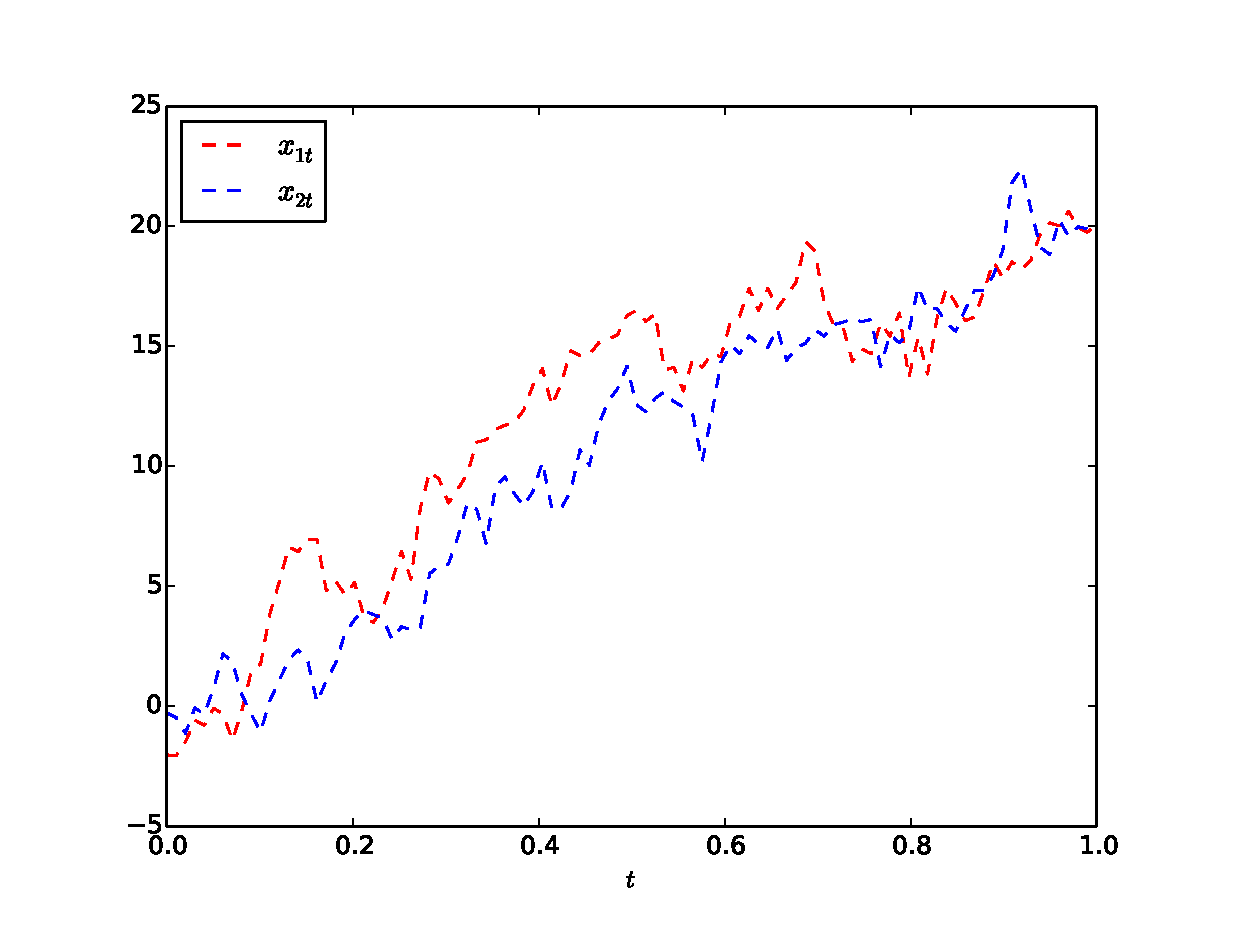
\includegraphics[width=0.8\textwidth]{img/spurious1}
  \caption{Two random walks time series $x_1,t$ and $x_2,t$}
  \label{fig:spurious1}
\end{figure}

\begin{figure}[!h]
  \centering
  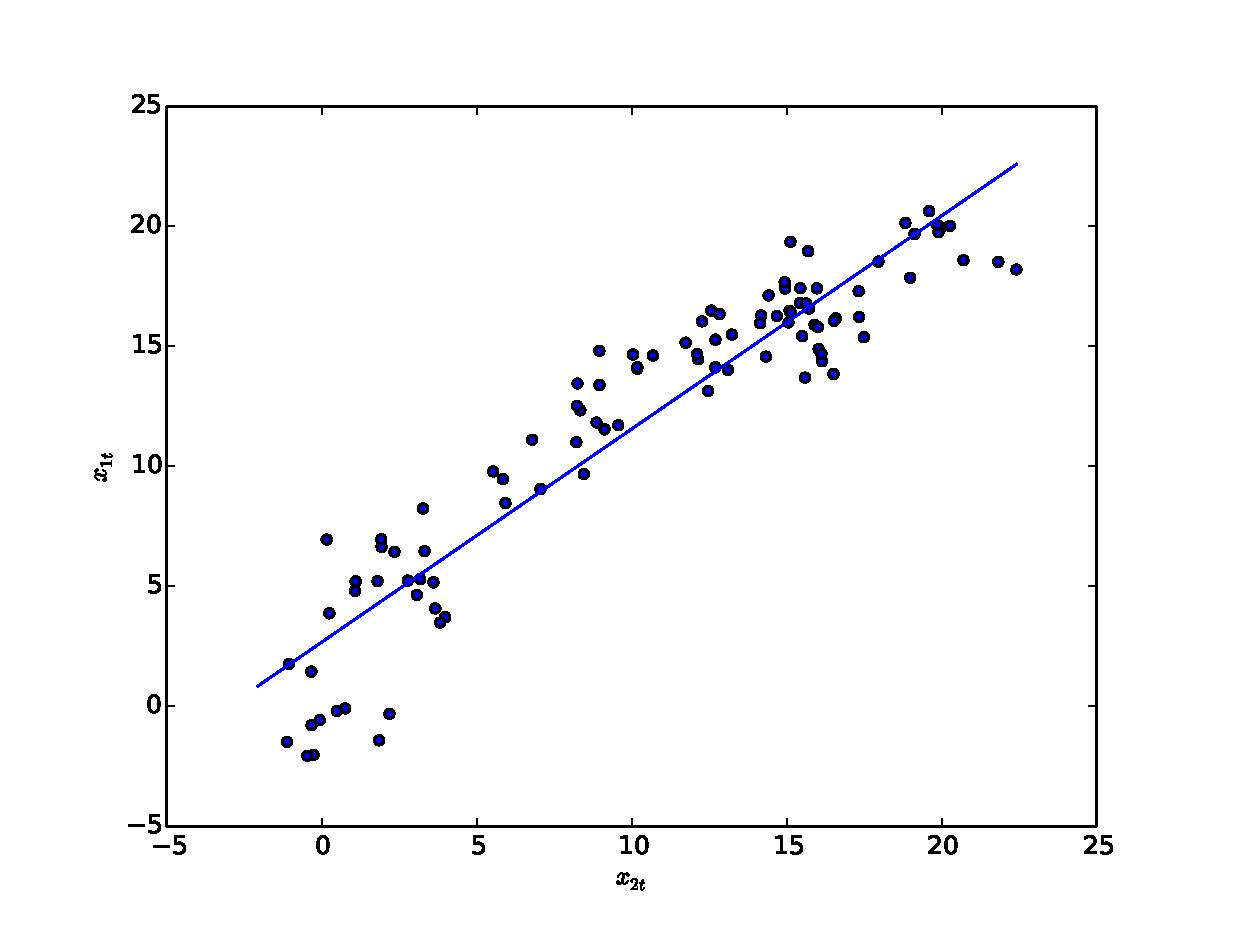
\includegraphics[width=0.8\textwidth]{img/spurious2}
  \caption{Regression between two random walks time series}
  \label{fig:spurious2}
\end{figure}

These two random walks, which are independent by construction, appear to be related with a $R^2=0.883$. However, what it is happening is that they are drifting in the same direction. Drift can be removed using returns or first differences.
If after taking returns or first differences the regression fit is still good we will say that the variables are cointegrated, this means that both series may drift but their residuals will not. A more formal definition of cointegration is given in the section \ref{sec:cointegration}.

%                            OLS Regression Results                            
%==============================================================================
%Dep. Variable:                      y   R-squared:                       0.883
%Model:                            OLS   Adj. R-squared:                  0.882
%Method:                 Least Squares   F-statistic:                     742.2
%Date:                Fri, 06 Feb 2015   Prob (F-statistic):           1.61e-47
%Time:                        06:07:47   Log-Likelihood:                -218.03
%No. Observations:                 100   AIC:                             440.1
%Df Residuals:                      98   BIC:                             445.3
%Df Model:                           1                                         
%==============================================================================
%                 coef    std err          t      P>|t|      [95.0% Conf. Int.]
%------------------------------------------------------------------------------
%x1             0.8883      0.033     27.243      0.000         0.824     0.953
%const          2.6726      0.405      6.606      0.000         1.870     3.475
%==============================================================================
%Omnibus:                        4.133   Durbin-Watson:                   0.363
%Prob(Omnibus):                  0.127   Jarque-Bera (JB):                4.145
%Skew:                          -0.469   Prob(JB):                        0.126
%Kurtosis:                       2.662   Cond. No.                         23.3
%==============================================================================

\newpage
\subsection{Integration}

Following Johansen \cite{johansen1995} we shall say that a stochastic process
$Y_t$ which satisfies $Y_t-E(Y_t) = \sum_{i=0}^\infty C_i\,\varepsilon_{t-i}$ is
called $I(0)$, and then we shall write $Y_t\sim I(0)$, whenever
$\sum_{i=0}^\infty C_i \neq 0$ and $\sum_{i=0}^\infty C_i\,z^i$ converges for
$z\in\mathbb{C}$ with $|z|<1$.  It is understood that the condition
$\varepsilon_t\sim iid(0,\sigma^2)$ holds.

A (vector) time series $\mathbf{y}_t$ is said to be {\em integrated of order\/}
$d$, and then we shall write $\mathbf{y}_t\sim I(d)$, whenever after $d$ times
(discrete) differentiation an stationary process is
obtained~\cite{banerjee1993};
more precisely, whenever
$(1-L)^d\,\mathbf{y}_t\sim\text{I(0)}$, where $L$ is the usual lag operator:
$(1-L)\,\mathbf{y}_t = \Delta\mathbf{y}_t = \mathbf{y}_t-\mathbf{y}_{t-1}$ for
all $t$.  

Note that this definition includes the scalar case as time series of
vectors of dimension 1; in this scalar case we will write the time series in
non-bold format.


\subsection{Cointegration} \label{sec:coint}
Cointegration concept was introduced by Engle in 1987 \cite{engle1987} and implies that one or
more linear combinations of non-stationary variables are stationary even though
individually they are not.  

Let $\mathbf{y}_t^\nu$, $\nu=1,\dots,p$, be a set of $p$ vector time series of
order $I(1)$.  They are said to be {\em cointegrated\/} if a vector
$\beta=[\beta(1),\dots,\beta(p)]^\top \in \mathbb{R}^p$ exists, such that the
time series,
\begin{equation}
\mathbf{Z}_t:= 
\sum_{\nu=1}^p \beta(\nu)\,\mathbf{y}_t^\nu\,\sim\,\text{I(0)}\,.
\end{equation}

In other words, a set of $I(1)$ time series is said to be cointegrated if a
linear combination of them exists, which is I(0).

Stock and Watson in 1988 \cite{stock+watson1988} observed that
cointegration reflects the common stochastic trends providing a useful way to
understand cointegration relationships. These common stochastic trends can be
also interpreted as a long-run equilibrium relationships.

The idea of cointegration was immediately adopted in finance since it could
represent their long-run relationship implied by economic
theory~\cite{laietAl1991}, \cite{lence+falk2005}.  Economic theory suggest that
economic time series are mean-reverting process and therefore, it reflects the
idea of that some set of variables cannot wander too far from each other. 

On the other hand, the efficient markets hypothesis, also known as the random
walk theory states that current stock prices fully reflect available information
related to its value and there is no way to earn excess profits~\cite{fama1970}.
This means that if we have stock prices from a jointly efficient market, they
cannot be cointegrated \cite{granger1986}, \cite{dwyer1992}. However,
\cite{richards1995} claims that cointegration is directly at odds with market
efficiency, even though, there is no evidence that cointegration among asset
prices have implications about market efficiency~\cite{lence+falk2005}.

Despite the fact that cointegration on closing daily rates of currency pairs has
not been found \cite{coleman1990}, \cite{copeland1991}, different time series
frequencies can have different behaviours~\cite{aldridge2009}. Pair trading is a
very common example of cointegration application~\cite{herlemont2003} but
cointegration can also be extended to a larger set of
variables~\cite{mukherjee1995},\cite{engle2004}.

\subsection{Johansen method}
Johansen in 1988 \cite{johansen1988} suggests a method for determining cointegration vectors. 

There are two statistics for cointegration under Johansen approach: the trace (shown in equation \ref{eq:johansentrace}) and the maximum-eigenvalue statistic (shown in equation \ref{eq:johansenmax}).

\begin{equation}
\label{eq:johansentrace}
\lambda_{\text{trace}} (r) = -T \sum_{i=r+1}^g \ln(1-\hat{\lambda_i})
\end{equation}


\begin{equation}
\label{eq:johansenmax}
\lambda_{\text{max}} (r,r+1) = -T \ln(1-\hat{\lambda_{r+1}})
\end{equation}


Where $r$ is the number of cointegration vectors and $\hat]{\lambda}_i$ is the estimated value for the ith ordered eigenvalue.  $\lambda_{\text{trace}}$ null hypothesis is that the number of cointegration vectors is less than or equal to $r$ against that there are more than $r$. $\lambda_{\text{max}}$ has the null hypothesis that the number of cointegration vectors is $r$ against an alternative of $r
+1$.


\newpage
\texttt{Cointegration example}

If we have two-dimensional process $\mathbf{X}_t$, $t=1,\dots,T$ by:

\begin{eqnarray*}
\mathbf{X}_{1t} &=& \sum_{i=1}^t \epsilon_{1i} + \epsilon_{2t} \\
\mathbf{X}_{2t} &=& a \sum_{i=1}^t \epsilon_{1i} + \epsilon_{3t} 
\end{eqnarray*}

Since $\mathbf{X}_{1t}$ and $\mathbf{X}_{2t}$ are I(1) processes and there
exist a vector $\beta = [a -1]$ such that:

\[
\beta^\top \mathbf{X}_t = a \mathbf{X}_{1t} -\mathbf{X}_{2t} = 
a\epsilon_{2t} - \epsilon_{3t} \sim \text{I(0)}
\]

then, both processes are said to be cointegrated. 


If we add a I(0) process
$\mathbf{X}_{3t} = \epsilon_{4t}$  we find that there exists two cointegration
vectors now: $\begin{bmatrix}a &-1& 0\end{bmatrix}$ and $\begin{bmatrix}0
&0&1\end{bmatrix}$ since:

\[
\beta^\top \mathbf{X}_t = 
\begin{bmatrix}
a & -1 & 0 \\
0 & 0 & 1
\end{bmatrix} 
\begin{bmatrix} 
\mathbf{X}_{1t} \\
\mathbf{X}_{2t} \\
\mathbf{X}_{3t}
\end{bmatrix} = 
\begin{bmatrix}
a\epsilon_{2t} - \epsilon_{3t} \\
\epsilon_{4t}
\end{bmatrix}
\]



\begin{figure}[!h]
  \centering
  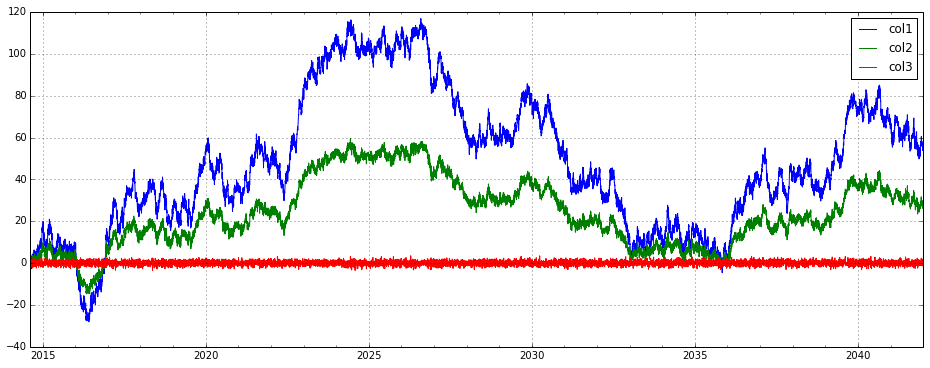
\includegraphics[width=\textwidth]{img/coint-example}
  \caption{Cointegration example: two processes I(1)(blue and green) and one process I(0) (red)}
  \label{fig:cointex}
\end{figure}

\begin{figure}[!h]
  \centering
 \begin{minipage}{\textwidth} %[b][\textheight][s]
  \centering
  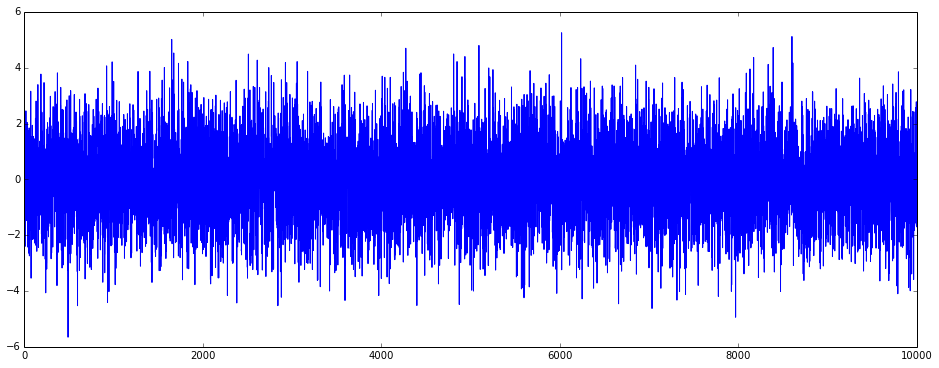
\includegraphics[width=0.9\textwidth]{img/coint-example2} 
   \caption{Time series linear combination using the first cointegration vector }
    \label{fig:cointvectors3}
   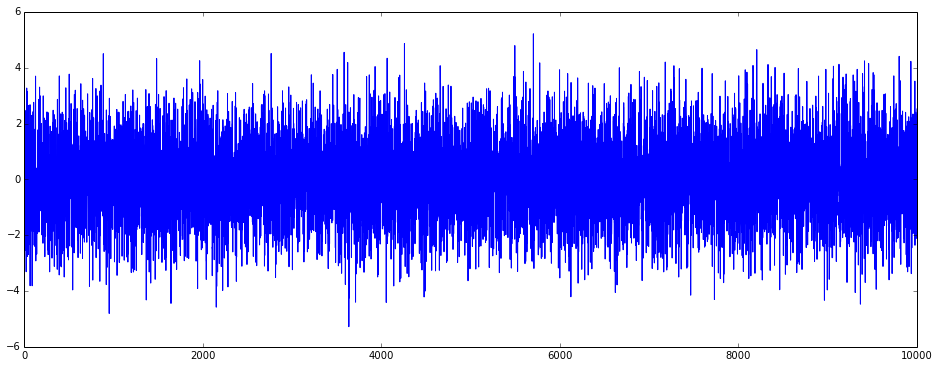
\includegraphics[width=0.9\textwidth]{img/coint-example3} 
    \caption{Time series linear combination using the second cointegration vector}
     \label{fig:cointvectors4}
    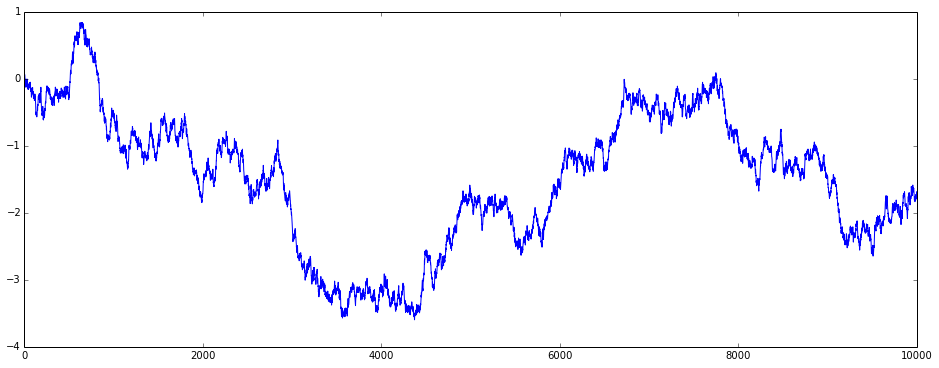
\includegraphics[width=0.9\textwidth]{img/coint-example4}
 \caption{Time series linear combination using the third cointegration vector}
   \label{fig:cointvectors5}
\end{minipage}
\end{figure}


This example shows how cointegration vectors describes the stable relations
between the processes by linear relations that are more stationary than the
original process. Cointegration vectors can be obtained using the Johansen method which gives with a certain probability the number of significant vectors. Figures    
\ref{fig:cointvectors3}, \ref{fig:cointvectors4}  and \ref{fig:cointvectors5}  shows the linear combinations obtained using cointegration vectors given by Johansen method. The method confirm that only two vectors are found and the third one given doesn't result in a I(0) process.


\section{Unit root tests}
Many economic and financial time series exhibit trending behaviour or non-stationary behaviour in the mean or variance. An important econometric task is to determine the type of non-stationary. For trend stationary I(0) time series a time-trend regression is appropriate. For I(1) time series taking first differences transforms it into a stationary one.  For cointegration to determine if time series are I(1) is mandatory to model their long-run relationship. In order to determine if a time series is an a I(1) or I(0) process unit root tests are used. Several tests have been developed but the most widely used is an extension of the Dickey and Fuller test \cite{dickey1979} called the Augmented Dickey-Fuller (ADF) test developed in 1984 by Said and Dickey in 1984\cite{said1984}.

The ADF test tests the null hypothesis that a time series $y_t$ is I(1) against the alternative that it is I(0), assuming that the dynamics in the data have an ARMA structure. The ADF test is based on estimating the test regression:

\begin{equation}
\label{eq:adftest}
y_t = \boldsymbol{\beta}^\top \mathbb{D}_t + \phi y_{t-1} + \sum_{j=1}^p \Psi_j \Delta y_{t-j} + \epsilon_t
\end{equation}

\noindent where $\mathbb{D}_t$ is a vector of deterministic terms. Lag length $p$ has to be determined when applying the test, Akaike Information Criteria (AIC) is commonly used to determine it.
The p-lagged difference terms $\Delta y_{t-j}$ are used to approximate an ARMA process and the value of $p$ is set so that the error $\epsilon_t$ is serially uncorrelated. 
Under the null hypothesis, $y_t$ is I(1) which implies that $\phi=1$. 
The test statistic is the following:

\[
\text{ADF}_t = \frac{\hat{\phi} -1}{SE(\phi)}
\]
\noindent where SE is the standard error.

The $\text{ADF}_t$ statistic is based on the least squares estimates of equation \ref{eq:adftest}.

\section{Stylized facts of asset returns}
\label{sec:stylizedfacts}

There are several known features exhibited by financial instruments called
stylized facts, which have been empirically studied and some of them have been
documented only recently and accepted as truth. Stylized facts are usually
formulated in terms of qualitative properties of asset returns and may not be
precise enough to distinguish among different parametric models.
\cite{cont2001}.

Returns of a time series $y$ is defined as:
\begin{equation}
\label{eq:returndef}
r_t = y_t - y_{t-1}  \, ,
\end{equation}

Some stylized facts which are common to a wide set of financial assets
\cite{sewell2011} are:

\begin{description}
\item[Dependence] autocorrelation in returns is largely insignificant. However,
autocorrelation in the absolute and squared returns is always positive and
significant and decays slowly. In addition, the autocorrelation in the absolute
returns is generally higher than the autocorrelation in the corresponding
squared returns. The returns autocorrelation function (ACF) of SPY is shown in figure
 \ref{fig:returnacf}. The figure shows how the correlations are significant even
 for very long lags, this imply that a long-memory process because of its
 long-range dependence. 
 \begin{figure}[h]
 \centering
 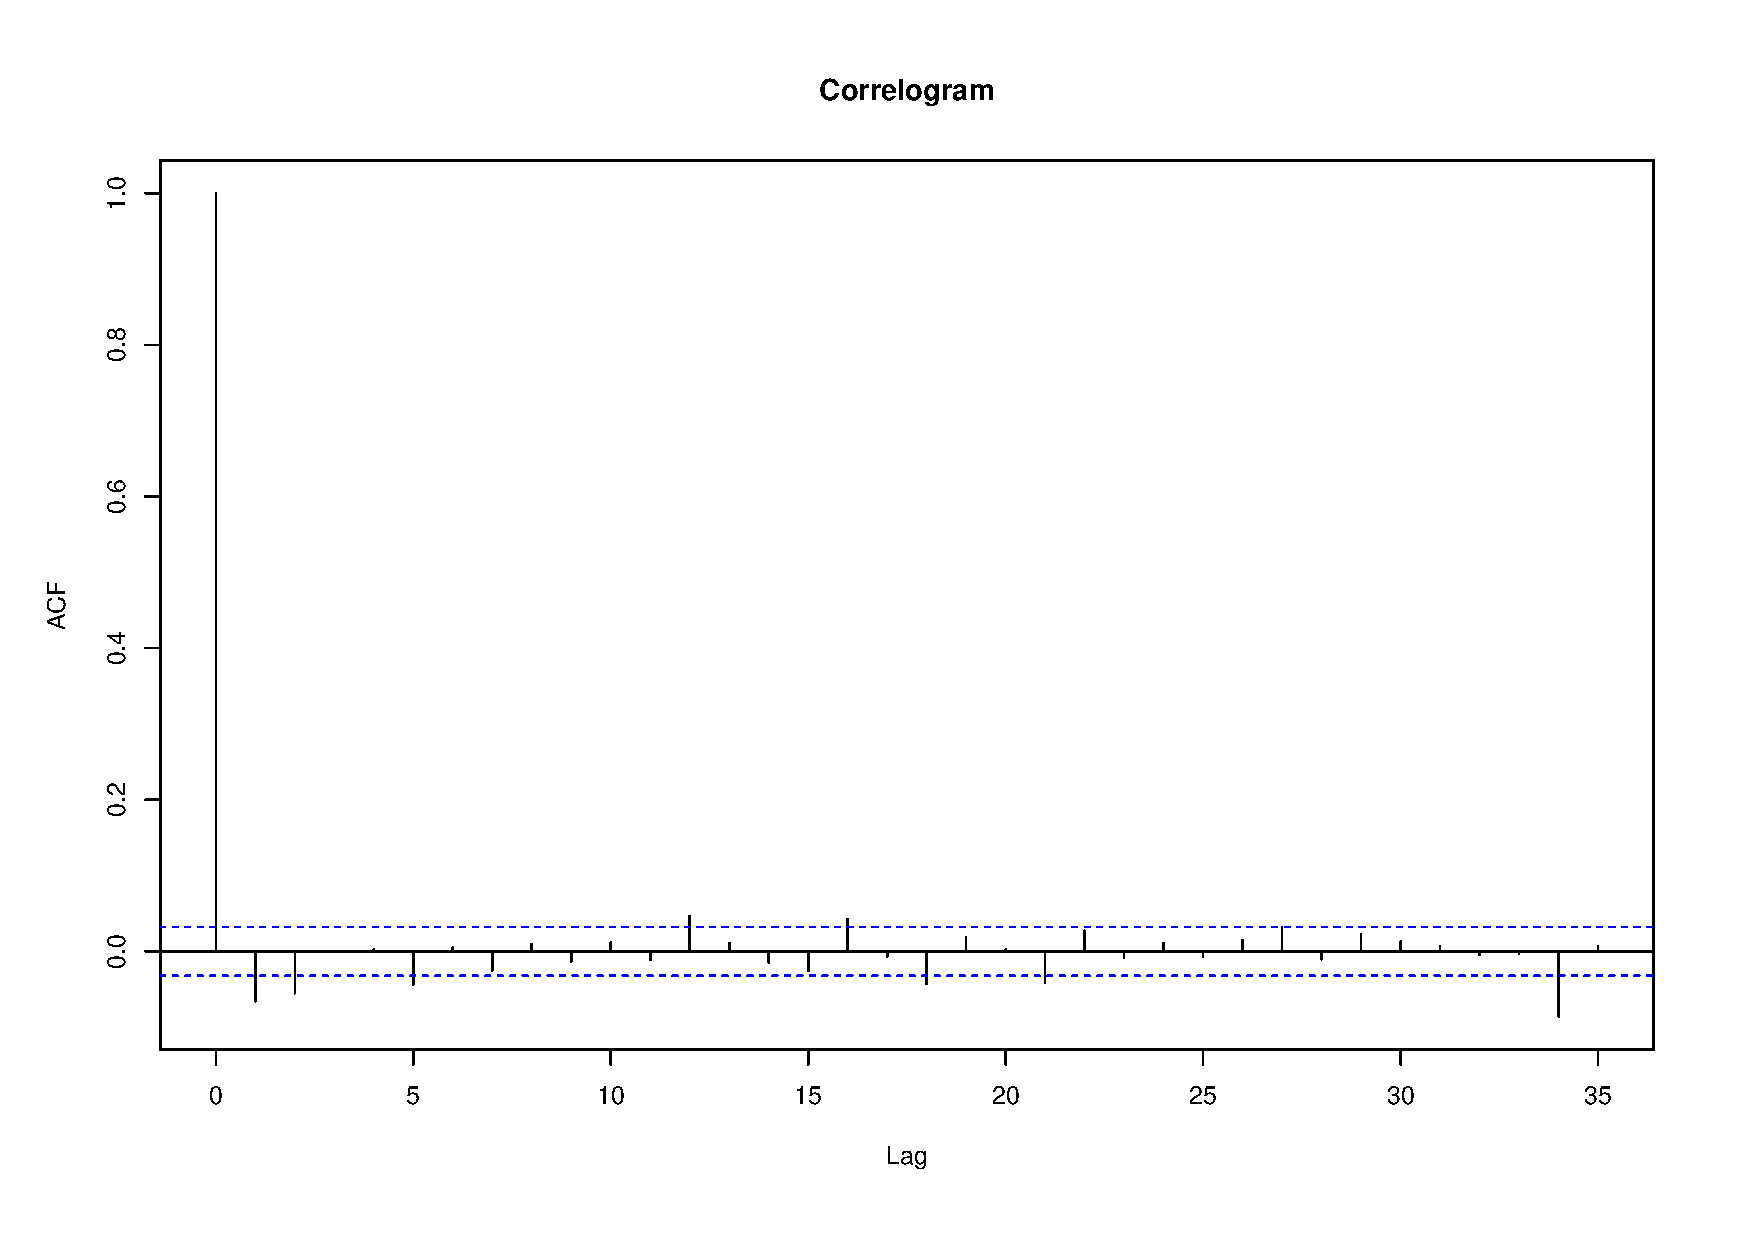
\includegraphics[width=0.7\textwidth]{plots/spy_returns_acf.pdf}
 \caption{SPY returns ACF}
 \label{fig:returnacf}
\end{figure}
\item[Distribution] The distribution of returns is approximately symmetric and
has high kurtosis (i.e fat tails and a peaked centre compared with the normal
distribution). However, distribution of returns whose were obtained from higher
frequencies looks more like a normal distribution.
The returns distribution tails are larger than
 what is hypothesised by common data generation process (generally normal
 distribution assumption). In the markets, fat tails are an undesirable feature
 because of the additional risk they imply.  In the figure \ref{fig:returndist}
 is shown the SPY returns distribution based on daily dates from the period 1st
 July 1998 to 4th April 2013. The distribution was compared against the normal
 distribution which clearly doesn't fit the data.  
 \begin{figure}[h]
 \centering
 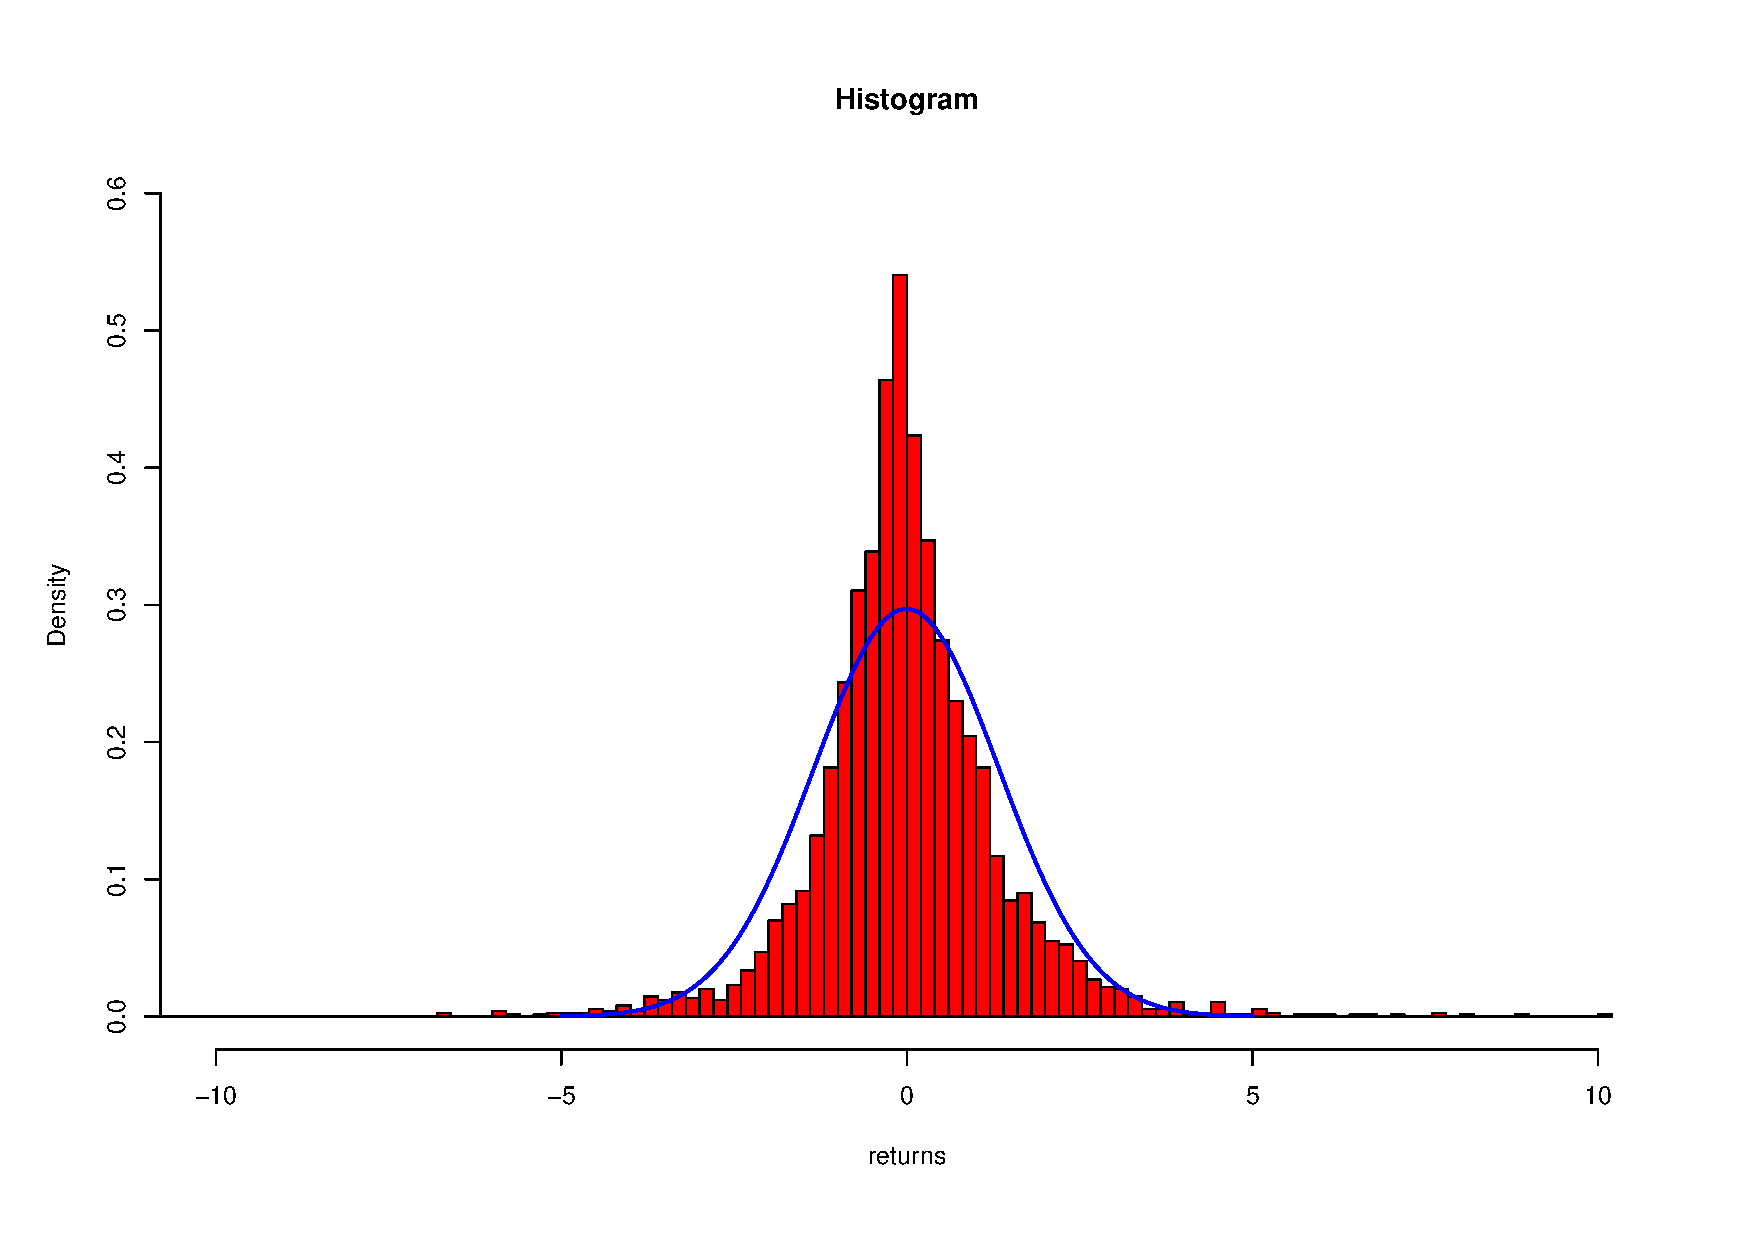
\includegraphics[scale=0.5]{plots/spy_returns_dist.pdf}
 % spy_returns_dist.pdf: 504x504 pixel, 72dpi, 17.78x17.78 cm, bb=0 0 504 504
 \caption{SPY returns distribution}
 \label{fig:returndist}
\end{figure}
\item[Heterogeneity] despite the fact that financial returns are non-stationary,
stationary periods can be observed. Economist speaks in terms of a structural
break \cite{stock1994}, in machine learning this is known as drift which means
that the statistical properties of the target variable change over time
\cite{widmer1996}, \cite{tsymbal2004}.
\item[Non-Linearity] financial returns may be non-linear in mean and/or
non-linear in variance.
\item[Calendar effects] are also called seasonal effects and they are cyclical
anomalies in returns where the cycle is based on the calendar. Some of known
calendar effects are: intraday effect, weekend effect, Monday effect, intramonth
effect, the January effect and Holiday effect. The most important calendar
anomalies are the January effect and the weekend effect. Figure
\ref{fig:mondayeffect} shows the Monday effect from 1928 to 2007. It shows that
in average Monday has negative returns. However, this is changing in time,
figure \ref{fig:mondayeffect2} shows returns only for year 2007 and its last
three months and it shows that Mondays and Wednesdays has positive returns in
average.

\begin{figure}[h!]
\centering
\begin{subfigure}[b]{0.45\textwidth}
 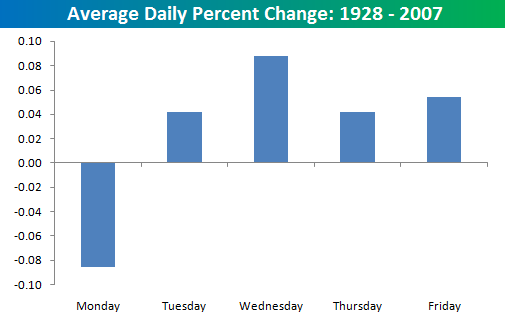
\includegraphics[width=\textwidth]{img/average_daily_change_1928_2007}
 \caption{Average daily return: 1928-2007}
 \label{fig:mondayeffect}
\end{subfigure}
\begin{subfigure}[b]{0.45\textwidth}
 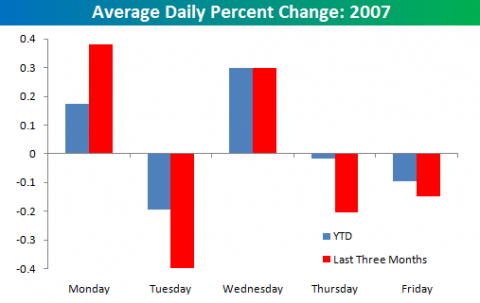
\includegraphics[width=\textwidth]{img/thumb-average_daily_change_2007}
 \caption{Average daily return: 2007}
 \label{fig:mondayeffect2}
\end{subfigure}
\end{figure}
\end{description}



\section{Volatility in the financial markets}
In financial markets, volatility is one of the key elements to model the
stochastic dynamic behaviour of financial assets. This is mainly because
volatility gives a measure of uncertainty about future returns and it is often
viewed as an indicator of the vulnerability of financial markets. It is also
important as an input parameter in problems like derivative pricing, hedging
and portfolio management.  For example, in option pricing we need to known
first the volatility of the underlying asset before pricing an option. 

Besides, volatility provides important information for studying asset returns
because the latter are largely uncorrelated and nonlinearly dependent. However,
it has been found that volatility exhibits significant autocorrelation and
predictable patterns~\cite{poon+granger2003} and  many models have been
proposed to forecast its behaviour. 

The volatility of the data is due to a large number of factors affecting the
market, with some of them directly measurable such as historical prices,
trends, supply and demand. However, others such as monetary policies and news
are not directly measurable and are included in other models out of the scope
of this thesis. 


Despite the fact variance and volatility are related, they are not the same concept. Variance is a measure of distribution of returns and is not necessarily
bound by any time period.  Volatility is a measure of the standard deviation
(square root of the variance) over a certain time interval. In finance,
variance and volatility both gives you a sense of an asset's risk. Variance
gives you a sense of the risk in the asset over its lifetime, while volatility
gives you a sense of the movement of the asset in, for example, the past month or the
past year. The main underlying difference is in their definition. Variance has a
fixed mathematical definition, however volatility does not as such. Volatility
is said to be the measure of fluctuations of a process.

Volatility is a subjective term, whereas variance is an objective term i.e.
given the data you can definitely find the variance, while you can't find
volatility just having the data. Volatility is associated with the process, and
not with the data. In order to know the volatility you need to have an idea of the process i.e you
need to have an observation of the dispersion of the process. All the different
processes will have different methods to compute volatilities based on the
underlying assumptions of the process.  

\subsection{Types of volatility}

The volatility of a stock is not directly observable~\cite{tsay2005,engle1993}. For example, daily volatility is not directly observable from only daily returns because there is only one observation in a trading day.  If intraday data is available, then volatility could be estimated. However, intraday returns are not the only explanatory variables for volatility and several estimators have been proposed. These estimators are observable variables that are related to the latent variable of interest called volatility proxies~\cite{devilderetal2007}. Examples of volatility proxies are the following: 



\subsubsection{realized volatility} is also known as historic volatility and
it is the actual variance in the price of a stock over time.
Realized volatility is measured in terms of the standard deviation
using the historical stock prices. It is commonly calculated based on
intraday price returns:
\begin{equation}
\label{eq:retintra}
r_{t,n}=100(\ln(p_{t,n}) - \ln(p_{t,n-1}))
\end{equation}
\noindent where $p_{t,n}$ is the price observed at day $t=1,\dots,T$ and
intraday sample $n=2,\dots,N$. Realized volatility is defined as:
\begin{equation}
\label{eq:rv}
    \hat{\sigma}(t) = \sum_{n=1}^N r_{t,n}^2 \, , 
\end{equation}
\noindent where $N$ is the number of intraday samples and $T$ is the
number of days. 
In order to include overnight returns, Hansen and
Lunde~\cite{hansen+lunde2005} introduced a scaling version of
realized volatility using the following definitions:
\begin{eqnarray}
r_{t}&=&100(\ln(p_{t,N}) - \ln(p_{t-1,N})) \label{eq: ret 1} \\
\bar{\rho}(t) &=& \sum_{t=1}^T r_{t}^2  \label{eq: ret 2} \, .
\end{eqnarray}
\noindent where equation~(\ref{eq: ret 1}) represents overnight 
returns and the volatility as 
equation~(\ref{eq: ret 2}), where $p_{t,N}$ is the last intraday 
sample at day $t$. The scaled realized volatility $\rho(t)$ is 
defined as:
\begin{eqnarray}
\label{eq:srv}
\rho(t) = \gamma \hat{\rho}(t) \, , \qquad & \qquad \gamma = \displaystyle \frac{\bar{\rho}(t)}{\displaystyle\sum_{t=1}^T \hat{\rho}(t)}
\end{eqnarray}
Realized volatility has also been defined as the absolute value return or as
the mean of the sum of intraday squared returns at short intervals of time. The
majority of research carried out in the literature obtain the daily volatility
as the daily squared returns as is shown in equation~(\ref{eq: ret 2}).
However, it has been proven that this measurement noise is too high for
observing the true volatility process~\cite{andersen+bollerslev1998}. Hansen
and Lunde~\cite{hansen+lunde2006} stated that the use of a noisy proxy could
result in an inferior model being chosen as the best one. The realized
volatility, as calculated by the cumulative sum of squared intraday returns and
shown in equation (\ref{eq:rv}), is less noisy and doesn't lead to choosing an
inferior model.   
\subsubsection{implied volatility volatility} not only can be extracted from returns
but it can also be derived from option or future pricing models.  The
volatility obtained corresponds to the market's prediction of future
volatility. In finance, an option is a derivative, that is, a contract which
gives the owner the right, but not the obligation to buy or sell an underlying
asset at a given price called strike price. An option can be executed at any
time before an expiration date previously defined no matter what price the
underlying asset has. For example, the Black-Scholes model~\cite{black1973}
determines the fair option value based on stock price, strike price, time to
option expiration, the interest rate and volatility. These are known or can be
easily obtained from the market, excepting by volatility which must be
estimated. However, rather than assuming a volatility a priori and computing
option prices from it, the model can be used to estimate volatility at given
prices, time to expiration and strike price. This obtained volatility is called
the implied volatility of an option. Additionally, some models obtain implied
volatility from futures (other derivative from prices). For instance, the
Barone-Adesi and Whaley futures option model~\cite{baroneetal1987} is also used
to determine future volatilities~\cite{hamidetal2004}. Higher implied
volatility is indicative of greater price fluctuation in either direction.
Implied volatility is found by determining the value which makes theoretical
prices equal to market prices. In this way volatility is ``implied'' by the
current market price of the stock.

In finance, an option is a derivative, that is, a contract which gives the owner
the right, but not the obligation to buy or sell an underlying asset at a given
price called strike price. An option can be executed at any time before an
expiration date previously defined no matter what price the underlying asset
has. 

The Black-Scholes formula~\cite{black1973}, developed in the early 1970's, Myron
Scholes, Robert Merton and Fisher Black,  allows to determine an option value
$V$ based on the underlying asset price $S(t)$ at a time $t$ and the following
constant parameters: 

\begin{description}
\item [$\sigma$:] underlying asset price volatility which measures the standard
deviation of the returns
\item [$\mu$:] underlying asset drift which is a measure of the average rate of
growth of the stock
\item[$E$:] option strike or excersice price
\item[$T$:] option date of expiry
\item[$t$:] current time
\item[$r$:] risk-free interest rate
\end{description}

The Black-Scholes model assume that the underlying price $S$ follows a lognormal random walk:

\begin{equation}\label{eq:stockprice}
dS = \mu S dt + \sigma S dB
\end{equation}

\noindent where $B$ is a Brownian motion. This stochastic differential equation
has two components: a deterministic term given by $\mu S dt$ and a random term
given by $\sigma S dX$.

A brownian motion $B$ (also called a Wiener process) is a stochastic process
characterized by the three following properties:

\begin{description}
\item[Continuity:] $B(t)$ is a continuos function
\item[Normal increments:]  $B(t)-B(s)$ has a normal distribution with mean $0$
and variance $t-s$.
\item[Independence of increments:] for every choice of nonnegative real numbers
$0 \leq s_1 <  t_1 \leq \cdots \leq s_n < t_n < \infty$, the increment random
variables $W_{t_1} - W_{s_1}, \cdots, W_{t_n} - W_{s_n}$ are jointly
independent.
\end{description}

An stochastic differential integral has the form:


\begin{equation}
W(T)=\int_0^T f(t)dB(t) \, .
\end{equation}

\noindent This equations is also expressed in an abbreviate form:

\begin{equation}
dW = f(t) dB \, .
\end{equation}

\noindent Therefore, the integral form of the stock price model shown in
equation (\ref{eq:stockprice}) is:

\begin{equation}
S(T)=\int_0^T \mu S(t) dt + \int_0^T \sigma S(t) dB(t)
\end{equation}


Ito's lemma is used to find the differential of a time dependent function of a
stochastic process. In option pricing we need to find the option price $V(S(t))$
which depends on a stochastic stock price model $S(t)$.  $V(S,t)$ is required to
be  differentiable function of $S$ and once differentiable function of $t$.

These are known or can be easily obtained from the market, excepting by
volatility which must be estimated. However, rather than assuming a volatility
a priori and computing option prices from it, the model can be used to estimate
volatility at given prices, time to expiration and strike price. This obtained
volatility is called the implied volatility of an option. Additionally, some
models obtain implied volatility from futures (other derivative from prices). 


For trading strategies, the interest is centred in forecasting realized
volatility over the life of an option and to take advantage when this
volatility differs from the implied volatility. This is called volatility
arbitrage. For example, a trader will buy an option and hedge the underlying
asset if the implied volatility is under the realized volatility. 


\subsection{Volatility methods}

In the existing literature, there are four main classes of asset
return volatility models: the general autoregressive conditional
heteroskedasticity (GARCH) models, the stochastic volatility (SV)
models, the realized volatility models and the machine learning based
models. A comparison of the first three models can be found
in~\cite{wei2012}. 

For many years the most popular methods for estimating financial
volatility were the autoregressive conditional heteroskedasticity
(ARCH) models~\cite{engle1982} and the general ARCH (GARCH)
models~\cite{bollerslev1986}. For instance, the GARCH(1,1) defines
returns $y_t$ and volatility $\sigma_t$ as:

\begin{eqnarray*}
    y_t &=& \sigma_t \epsilon_t \\
     \sigma_t^2 &=& \alpha_0 + \alpha_1 \epsilon_{t-1}^2 + \beta_1
     \sigma_{t-1}^2
\end{eqnarray*}

\noindent where $\epsilon_t$ is standard Gaussian white noise,
$\alpha_0,\alpha_1,\beta_1 \geq 0$ are required to ensure that the
variance will never be negative and $\alpha_1+\beta_1 <1$ is needed to
guarantee a weakly stationary process~\cite{nelson1990}.

Since the introduction of the GARCH models, several extensions have been
proposed, but none of them seems to beat the GARCH(1,1)
model~\cite{lunde+hansen2005}. Despite its popularity, GARCH models have
several limitations: firstly, a time series model may be non-linear in mean
and/or non-linear in variance, but ARCH and GARCH models are non-linear in
variance, but not in mean. Besides, GARCH models often fail to capture highly
irregular phenomena, like wild market fluctuations.  

SV models explain how volatility varies in a random fashion. These models are
useful because they explain why options with different strikes and expirations
dates have different Black-Scholes implied volatilities, phenomenon known as
the volatility smile. This is useful because the Black-Scholes model assumes
that the volatility of the underlying asset is constant which is not always
true. There are several SV models and the most well-known and popular is the
Heston model~\cite{heston1993}. Additional information about SV models can be
found in~\cite{shephard1995}. 

The realized volatility constructed from high frequency intraday returns gave
rise to the realized volatility models mainly because the realized volatility
series is much more homoskedastic and seems to be a long memory
process~\cite{andersonetal2003}. For realized volatility, the autoregressive
fractionally integrated moving average (ARFIMA) process emerged as a standard
model~\cite{chenetal2010} and many variations have been studied, but all of
them produce similar forecasting results to the ARFIMA(1,d,1)
model~\cite{koopmanetal2005}.  

On the other hand, machine learning based models, especially artificial neural
networks (ANN) and support vector machines (SVM) have arisen as an alternative
to forecast volatility. ANN is a statistical technique inspired by biological
neural networks which is capable of changing its structure based on external or
internal information during a training phase~\cite{sammut2011}. SVM are
supervised learning models for classification analysis which recognize patterns
finding a separating hyperplane. An extension for regression analysis is known
as support vector regression (SVR). 

Since machine learning models and in particular ANN do not require assumptions
about the data (gaussianity for example) and allow more explanatory variables
than returns to be included, they have become widely used in solving financial
problems, specially volatility
forecasting~\cite{hamidetal2004,donaldsonetal1997}. There are also many works
focused on the using of SVM in volatility
forecasting~\cite{shiyietal2008,shiyietal2010,gavrishchaka2006,vasilios2012}. 

However, just as with ANN, SVMs have scalability problems because their
training process is computationally intensive and it is done in batch mode. The
scalability problem worsens when new additional training data is available and
a re-training process from scratch needs to be done. This problem can be
avoided using online machine learning algorithms that allow one instance at a
time to be processed with low computationally expensive calculations.



\section{Vector Autoregressive Models}\label{sec:varvec}

The vector autoregressive VAR($p$) model is one of the most easy to use, successful and flexible models for the analysis of multivariate time series. It is a natural extension of the univariate autoregressive (AR) model. The VAR model has proven to be useful for describing the dynamic behaviour of economic and financial time series.
VAR is a general framework describing the behaviour of a
set of $l$ endogenous variables as a linear combination of their last $p$
values, where $l,p\in\mathbb{N}$. 
In our case, each one of these $l$ variables is a scalar time series
$y_{\lambda,t}$, $\lambda=1,\dots,l$, and we represent them all together
at time $t$ by the the vector time series:
\begin{equation}
\label{eq:variables}
\mathbf{y}_t = 
\begin{bmatrix} y_{1,t} & y_{2,t} & \dots & y_{l,t} \end{bmatrix}^\top.
\end{equation}
\noindent
Notice that the vectors $\mathbf{y}_t$ are assumed to be $l$-dimensional.

The VAR($p$) model describes the behaviour of a dependent variable in terms of
its own lagged values and the lags of the others variables in the system. The
model with $p$ lags is formulated as the system of $N$:
\begin{align}
\label{eq:var}
\mathbf{y}_t 
= \boldsymbol{\Phi}_1 \mathbf{y}_{t-1} +
  \boldsymbol{\Phi}_2 \mathbf{y}_{t-2} + \dots +
  \boldsymbol{\Phi}_p\mathbf{y}_{t-p} +
  \mathbf{c} + \boldsymbol{\epsilon}_t \nonumber \\
t=p+1,\dots,N,
\end{align}
\noindent where 
$\boldsymbol{\Phi}_1, \boldsymbol{\Phi}_2,\dots,\boldsymbol{\Phi}_p$
are $l\times l$-matrices of real coefficients,
$\boldsymbol{\epsilon}_{p+1},
 \boldsymbol{\epsilon}_{p+2}, \dots, \boldsymbol{\epsilon}_N$ 
are error terms, $\mathbf{c}$ is a constant vector and $N$ is the total
number of samples.

Notice that, regarding our notation of section (\ref{sec:coint}),
we have here 
$\mathbf{y}_t^0 = \mathbf{y}_t$,
$\mathbf{y}_t^\nu = \mathbf{y}_{t-\nu}$ and
the $\lambda$-th component of the vector time series $\mathbf{y}_t^\nu$
is the scalar time series $y_{\lambda,t}^\nu$, where $\nu=1,\dots,p$ and
$\lambda=1,\dots,l$.
Transposing each equation of the system (\ref{eq:var}) we can write
the VAR($p$) model in block-matrix form as:
\begin{equation}\label{eq:vareq}
\mathbf{B} = \mathbf{A} \mathbf{X} + \mathbf{E} \, , 
\end{equation}
%%
\noindent where:
%%
\begin{alignat}{2}
\mathbf{B}
&= \begin{bmatrix}
   \mathbf{y}_{p+1}^\top \\
   \mathbf{y}_{p+2}^\top \\
   \vdots \\
   \mathbf{y}_N^\top
   \end{bmatrix}_{(N-p)\times l}
&\quad
\mathbf{A}
&= \begin{pmat}[{...|}]
   \mathbf{y}_p^\top & \mathbf{y}_{p-1}^\top & \dots 
                    & \mathbf{y}_1^\top & 1 \cr
   \mathbf{y}_{p+1}^\top & \mathbf{y}_p^\top & \dots
                       & \mathbf{y}_2^\top & 1 \cr
   \vdots & \vdots & \ddots & \vdots & \vdots \cr
   \mathbf{y}_{N-1}^\top & \mathbf{y}_{N-2}^\top & \dots 
                       & \mathbf{y}_{N-p}^\top & 1 \cr
   \end{pmat}_{(N-p)\times(pl+1)} \\
\mathbf{X}
&= \begin{bmatrix}
   \boldsymbol{\Phi}_1^\top \\
   \boldsymbol{\Phi}_2^\top \\
   \vdots \\
   \boldsymbol{\Phi}_p^\top \\
   \mathbf{c}^\top
   \end{bmatrix}_{(pl+1)\times l}
&\quad
\mathbf{E}
&= \begin{bmatrix}
   \boldsymbol{\epsilon}_{p+1}^\top \\
   \boldsymbol{\epsilon}_{p+2}^\top \\
   \vdots \\
   \boldsymbol{\epsilon}_N^\top \\
   \end{bmatrix}_{(N-p)\times l}
\end{alignat}
Taking into account the error term $\mathbf{E}$, equation~(\ref{eq:vareq}) 
can be solved with respect to $\mathbf{X}$ using the ordinary least
squares estimation.

\section{Vector error correction model}
Vector error correction model (VECM) is a special form of a VAR model for I(1) variables that are also
cointegrated~\cite{banerjee1993}.

It is obtained re-writing equation (\ref{eq:var}) in terms of the new
variable $\Delta\mathbf{y}_t=\mathbf{y}_t-\mathbf{y}_{t-1}$.
The VECM model, expressed in terms those differences, takes the form:
\begin{equation}\label{eq:vec}
\Delta \mathbf{y}_t 
= \boldsymbol{\Omega}\,\mathbf{y}_{t-1}
  + \sum_{i=1}^{p-1} \boldsymbol{\Phi}_i^*\,\Delta\mathbf{y}_{t-i}
  + \mathbf{c} + \boldsymbol{\epsilon}_t\,,
\end{equation}
\noindent
where the coefficients matrices $\boldsymbol{\Phi}_i^*$ and 
$\boldsymbol{\Omega}$, expressed in terms of the matrices
$\boldsymbol{\Phi}_i$ of (\ref{eq:var}), are:
\begin{align*}
\boldsymbol{\Phi}_i^* 
&:= -\sum_{j=i+1}^{p}\boldsymbol{\Phi}_j\,, \\
\boldsymbol{\Omega}
&:= -\left( \mathbb{I} - \boldsymbol{\Phi}_1 - \dots 
    - \boldsymbol{\phi}_p \right)\,. 
\end{align*}
The following well known properties of the matrix $\boldsymbol{\Omega}$
\cite{johansen1995} will be useful in the sequel:
\begin{itemize}
\item
If $\boldsymbol{\Omega} = \mathbf{0}$, there is no cointegration.
\item 
If $rank(\boldsymbol{\Omega})=l$, i.e., if $\boldsymbol{\Omega}$ has
full rank, then the time series are not I(1) but stationary.
\item
If $rank(\boldsymbol{\Omega})=r$, $0<r<l$, then there is cointegration
and the matrix $\boldsymbol{\Omega}$ can be expressed as
$\boldsymbol{\Omega}=\boldsymbol{\alpha\beta}^\top$, where $\boldsymbol{\alpha}$
and $\boldsymbol{\beta}$ are
$l\times r$ matrices and
$\text{rank}(\boldsymbol{\alpha})=\text{rank}(\boldsymbol{\beta})=r$.
\item
The columns of $\boldsymbol{\beta}$ contains the cointegration vectors and the rows of
$\boldsymbol{\alpha}$ correspond with the adjusted vectors. 
$\boldsymbol{\beta}$ is obtained by Johansen procedure~\cite{johansen1988},
whereas $\boldsymbol{\alpha}$ has to be determined as a variable in the VECM.
\end{itemize}
It is worth noticing that the factorization of the matrix
$\boldsymbol\Omega$ is not unique, since for any $r \times r$
nonsingular matrix $\mathbf{H}$, $\boldsymbol{\alpha}^*:=\boldsymbol{\alpha}\mathbf{H}$,
and $\boldsymbol{\beta}^*=\boldsymbol{\beta}(\mathbf{H}^{-1})^\top$ we have
$\boldsymbol{\alpha\beta}^\top=\boldsymbol{\alpha}^*(\boldsymbol{\beta}^*)^\top$.
If cointegration exists, then equation (\ref{eq:vec}) can be written
as follows:
\begin{equation}\label{eq:vecfull}
\Delta\mathbf{y}_t 
= \boldsymbol{\alpha\beta}^\top\mathbf{y}_{t-1} 
  + \sum_{i=1}^{p-1}\boldsymbol{\Phi}_i^*\,\Delta\mathbf{y}_{t-i}
  + \mathbf{c} + \boldsymbol{\epsilon}_t\,,
\end{equation}
\noindent
which is a VAR model but for time series differences.


Transposing each equation of the system (\ref{eq:vecfull}) we can write
the VECM($p$) model in block-matrix form as:
\begin{equation}\label{eq:vareq}
\mathbf{B} = 
\mathbf{A} \mathbf{X} + 
\mathbf{E} \, , 
\end{equation}
%
\noindent where $\mathbf{B}$ dimension is $((N-p)\times l)$, $\mathbf{A}$
dimension is $((N-p)\times(r+(p-1)l +1))$, $\mathbf{X}$ dimension is $((r+(p-1)l
+1)\times l)$ and $\mathbf{E}$ dimension is $((N-p)\times l)$:
%
\begin{alignat}{3}
\mathbf{B}
&= \begin{bmatrix}
   \Delta\mathbf{y}_{p+1}^\top \\
   \Delta\mathbf{y}_{p+2}^\top \\
   \vdots \\
   \Delta\mathbf{y}_N^\top
   \end{bmatrix}
&\quad
\mathbf{X}
&= \begin{bmatrix}
   \boldsymbol{\alpha}^\top \\
   \boldsymbol{\Phi}_1^{*\top} \\
   \boldsymbol{\Phi}_2^{*\top} \\
   \vdots \\
   \boldsymbol{\Phi}_{p-1}^{*\top} \\
   \mathbf{c}^\top
   \end{bmatrix}
&\quad
\mathbf{E}
&= \begin{bmatrix}
   \boldsymbol{\epsilon}_{p+1}^\top \\
   \boldsymbol{\epsilon}_{p+2}^\top \\
   \vdots \\
   \boldsymbol{\epsilon}_N^\top \\
   \end{bmatrix}
\end{alignat}
\noindent and 
\begin{align}
\mathbf{A}
&= \begin{pmat}[{....|}]
   \mathbf{y}_p^\top \boldsymbol{\beta} & \Delta \mathbf{y}_p^\top & \Delta\mathbf{y}_{p-1}^\top & \dots 
                    & \Delta\mathbf{y}_2^\top & 1 \cr
   \mathbf{y}_{p+1}^\top  \boldsymbol{\beta} &\Delta\mathbf{y}_{p+1}^\top & \Delta\mathbf{y}_p^\top & \dots
                       & \Delta\mathbf{y}_3^\top & 1 \cr
   \vdots & \vdots & \vdots & \ddots & \vdots & \vdots \cr
   \mathbf{y}_{N-1}^\top  \boldsymbol{\beta} &\Delta\mathbf{y}_{N-1}^\top & \Delta\mathbf{y}_{N-2}^\top & \dots 
                       & \Delta\mathbf{y}_{N-p-1}^\top & 1 \cr
   \end{pmat}\, .
\end{align}
Taking into account the error term $\mathbf{E}$, equation~(\ref{eq:vareq}) 
can be solved with respect to $\mathbf{X}$ using the ordinary least
squares estimation (see section \ref{sec:OLS}).

VECM models are employed because many economic time series appear to be first-difference stationary, i.e. I(1)

Conventional regression estimators, including VARs, have good properties when applied to covariance-stationary time series, but encounter difficulties when applied to non stationary or integrated processes.

These difficulties were illustrated by Granger and Newbold in 1974 \cite{granger1974} when they introduced the concept of spurious regressions (see section \ref{sec:spurious}). In 1982, Nelson and Plosser  \cite{nelson1982} showed that unit roots might be present in a wide variety of macroeconomic series
in levels or logarithms. This finding gave rise to the industry of unit root testing, and
the implication that variables should be rendered stationary by
differencing before they are included in an econometric model.
Further theoretical developments by Granger and Engle in 1987 \cite{engle87} raised the possibility that two or more integrated, non stationary time series might be cointegrated, so that some linear combination of these series could be stationary even though each series were not. 

If two series are both integrated (of order one, or I(1)) we could model
their interrelationship by taking first differences of each series and
including the differences in a VAR or a structural model.
However, this approach would be suboptimal if it was determined that
these series are indeed cointegrated. In that case, the VAR only
express the short-run responses of these series to innovations in each
series. This implies that the simple regression in first differences is
misspecified.
If the series are cointegrated, they move together in the long-run. A
VAR in first differences will not capture those long-run tendences.
VECM fit to the first differences of the non stationary variables, but a lagged error-correction term is added to the relationship representing the long-run relationship.

\subsection{Ordinary Least Squares method} \label{sec:OLS}

The solution $\widehat{\mathbf{A}}$ to
equation~(\ref{eq:vareq}) can be obtained by the ordinary least squares (OLS)
method. $\widehat{\mathbf{X}}$ is the solution of the quadratic optimization problem
\begin{equation*}
\widehat{\mathbf{X}} = \underset{\mathbf{X}}{\text{Arg\;min}}
\|\mathbf{A}\mathbf{X}-\mathbf{B}\|_2^2
\end{equation*}
\noindent for which the solution $\widehat{\mathbf{X}}$ is well-known:
\begin{equation*}
\label{eq:MP}
\widehat{\mathbf{X}}=\mathbf{A}^{\!\!+}\,\mathbf{B}
\end{equation*}
\noindent where $\mathbf{A}^{\!\!+}$ is the Moore-Penrose pseudo-inverse
which, when $\mathbf{A}$ is full rank, can be written as follows: 
\begin{equation}
\label{eq:pseudoinverse}
\mathbf{A}^{\!\!+}= (\mathbf{A}^{\!\!\top} \mathbf{A})^{-1}\mathbf{A}^{\!\!\top} \, .
\end{equation}
when $\mathbf{A}$ is not full rank, i.e
$rank(\mathbf{A})=k <  n \leq m$, $\mathbf{A}^\top \mathbf{A}$ is
always singular and equation~(\ref{eq:pseudoinverse}) cannot be used.
More generally, the pseudo-inverse is best computed using the compact
singular value decomposition (SVD) of $\mathbf{A}$ which is:
%\begin{equation}
%    \label{eq:compactsvd}
%    \underset{m \times n}{\mathbf{A}}=
%    \underset{m \times k}{\mathbf{U_1}} \enskip
%    \underset{k \times k}{\Sigma_1} \enskip
%    \underset{k \times n}{\mathbf{V}_1^{\top}} \, .
%\end{equation}
\begin{equation*}
    \label{eq:compactsvd}
    \mathbf{A}=
    \mathbf{U_1}
    \boldsymbol \Sigma_1
    \mathbf{V}_1^{\top} \, .
\end{equation*}
Pseudo-inverse can then be written as follows:
\begin{equation*}
\label{eq:pseudoinversesvd}
\mathbf{A}^{\!\!+} = \mathbf{V}_1 \boldsymbol \Sigma_1^{-1} \mathbf{U}_1^\top \, .
\end{equation*}


